Query 1 requires us to forecast the average load of each plug and each house in the system for different time windows of length 1,5,15,60,120 min. The average load forecast is computed over all possible slots of all the time slices. In order to make a forecast for the next to next slot, we use two values - current average load and median load of the corresponding slot of given time slice. We put out a forecast every 30 sec i.e. for each time slice we compute average load whenever we accumulate data for next 30 seconds.

\subsection{Architecture}
The system consists of a broker process and multiple house processes (one per house). The broker reads the data file and creates an event stream for each house process. The house processes are responsible for forecasting average load of the house and all plugs in the house.

In house processes for each plug, we keep a 30 second accumulator and counter. Whenever we receive an event for a plug, we increment the accumulator with the load\footnote{For now, we are ignoring events with work values} value in the received event and increment the counter for computing the average load later. We also keep load value accumulators and counters for different time slices (1m, 5m, 15m, 60m and 120m). As soon as we receive an event crossing the 30s time window, we add the 30s accumulator \& counter value to each time slice variables, compute \& output the forecast for all time slices and reinitialize the 30s accumulator \& counter to the load value in the received event \& 1 respectively. If any of the time slice boundaries are crossed, corresponding accumulators and counters are reset to 0. We output the forecast as zero if all the data is missing in a slot for a time slice. Note that, the above algorithm is based on the assumption that the timestamp of events coming from the broker never decreases. We, therefore, can make the forecast whenever any event corresponding to any plug in the house, crossing the current time slot for a time slice is received. We do a similar computation for house average load forecast.

We designed a Median Container (MC) to compute exact median of average load for a given slot of fixed time slice in case of query 1. The MC provides an interface to insert a new element and retrieve the median of all the elements currently in the container. For this, MC uses a min heap, max heap and a middle variable. The min heap holds the upper half of the inserted values and max heap holds the lower half. If the number of values in the container is odd the middle variable keeps the median, otherwise the median is the average of the top of max heap and min heap. New entries are added while carefully maintaining the above specified property. The asymptotic complexity of insert is $O(\log N)$ whereas median can be retrieved in constant time.

\subsection{Prediction Model}
We have used Weighted Average with Adaptive Weights prediction model in order to forecast the average load of a house or a plug. The \textit{Predicted Average Load} (PL) for a given time slot of a given time slice is computed as follows-
\begin{align*}
\mbox{PL} &= \mbox{W}*\mbox{HM}  + (1-\mbox{W})*\mbox{CA}
\end{align*}

\noindent Where HM (\textit{History Median}) is the median of average loads of previous days for the same time slot of same time slice and W is the weight that we are assigning to HM in comparison with \textit{Current Average} (CA). We make the prediction for next time slot of same time slice.
Hence, CA is the average of last time slot.
We give equal weights to HM and CA in the beginning and set the initial value of the weight \textit{W} as 0.5. As the program execution progresses, the value of \textit{W} is adapted based on the actual value we receive for each output forecast.
We define the error in the forecast as follows-
\begin{align*}
\mbox{Error} &= (\mbox{AL} - \mbox{PL})^2 + \lambda * (\mbox{W}_{new} - \mbox{W})^2
\end{align*}

\noindent $\lambda$ is a parameter to control the learning over W, AL is \textit{Actual load} and PL (\textit{Predicted Average Load}) is computed using $\mbox{W}_{new}$.
Our goal is to minimize the above Error.
We differentiate Error with respect to $\mbox{W}_{new}$ and get the following expression when equated to 0.
\begin{align*}
\mbox{W}_{new} &= \frac{\mbox{W}*\lambda-(\mbox{AL}-\mbox{CA}) * (\mbox{HM}-\mbox{CA})}{\lambda + (\mbox{HM}-\mbox{CA})^2}
\end{align*}

Note that we use different weights for different houses for each time slice. We tried different values of $\lambda=0.01, 2, 100$ and achieved minimum error in case of $\lambda = 2$. $\lambda$ is kept fixed throughout the experiment.

\subsection{Experimental Evaluation}
We executed our solution on a cluster of KVM virtual machines. The broker runs on a single core 2.1 GHz virtual machine with 1 GB memory and attached to a 10 Gbit local area network. The virtual machine is running Ubuntu 12.04 on dual processor Intel Xeon E5 2620 base system.
The house processes also run on a similarly configured virtual machines. We have done experiments running house processes on 1,2 and 4 virtual machines dividing the number of house processes equally amongst the VMs. For throughput calculations, we redirected the output to the null device. Throughput will simply be the total number of input events divided by the total time taken in processing all the events.
We did each experiment three times and took the average of the three throughput values.

\begin{figure}[h]
\begin{center}
	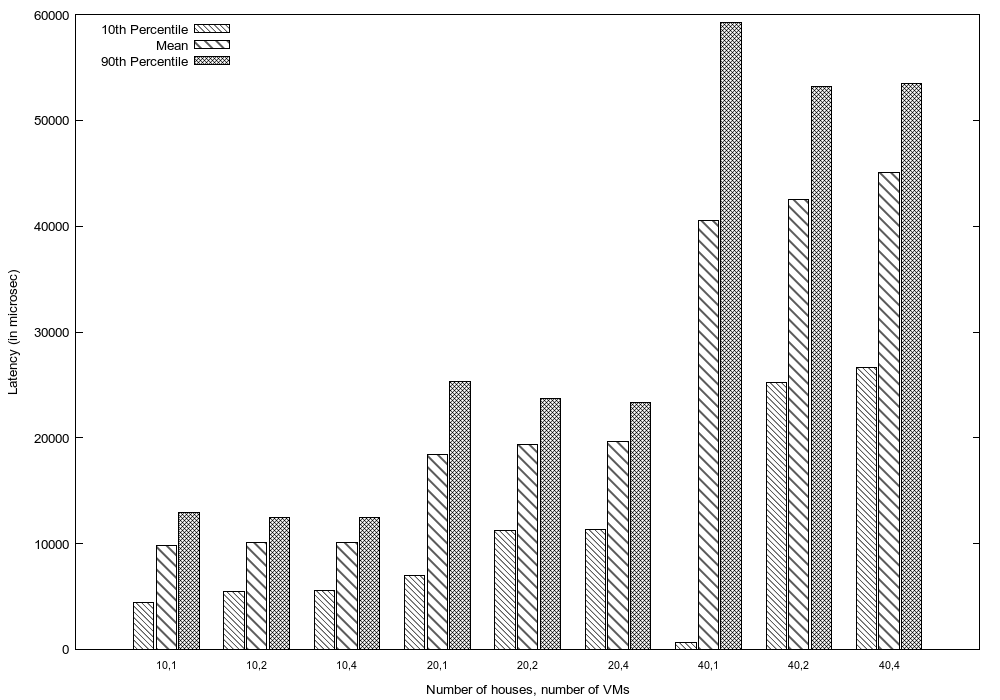
\includegraphics[width=0.4\textwidth]{img/q1_latency}
	\vspace*{-0.4cm}
	\caption{Latency vs No of Houses (Query 1) \label{fig:q1_latency}}
\end{center}
\vspace*{-0.3cm}
\end{figure}

As we increase the number of virtual machines, the latency values do not change much as shown in Figure \ref{fig:q1_latency} because the broker becomes the bottleneck. But latency increases as the number of houses increases, this is because of additional events between two events of same house. On the other hand, throughput remains nearly constant in all the experiments as shown in Figure \ref{fig:q1_throughput}.

We contend based on utilization of CPU at the broker; house processes consume little of CPU. It is the broker that is currently limiting the scalability of the system. The parsing of the read event accounts for most of the time spent by the broker on the CPU.
If we were getting events as a stream and can avoid both the disk I/O and conversion of strings to numbers, we can witness the scalability of the system as a whole since the house processes are separate and can be run on different cores.

\begin{figure}[h]
\begin{center}
	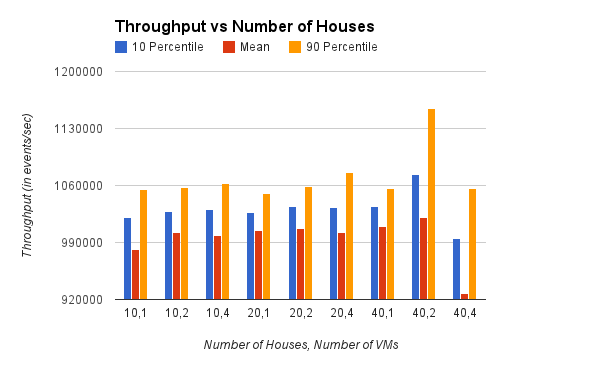
\includegraphics[width=0.4\textwidth]{img/q1_throughput}
	\vspace*{-0.4cm}
	\caption{Throughput vs No of Houses (Query 1)\label{fig:q1_throughput}}
\end{center}
\vspace*{-0.4cm}
\end{figure}
